\documentclass{article}

\usepackage{spconf,amsmath,graphicx,booktabs,cite}


\name{Seunghun Oh$^{1}$\qquad
Hyunjung Chung$^{2}$\qquad
Ganghyeon Jeong$^{1}$\qquad
Unsang Park$^{1,2}$%
\sthanks{\begingroup\fontsize{9}{10.2}\selectfont
Corresponding author: Unsang Park.\endgroup}}
        
\address{$^{1}$Department of Artificial Intelligence, Sogang University, Seoul, Republic of Korea\\
  $^{2}$Department of Computer Science and Engineering, Sogang University, Seoul, Republic of Korea}

\renewcommand{\topfraction}{0.92}
\renewcommand{\bottomfraction}{0.85}
\renewcommand{\textfraction}{0.06}
\renewcommand{\floatpagefraction}{0.80}
\renewcommand{\dbltopfraction}{0.92}
\renewcommand{\dblfloatpagefraction}{0.80}
\setlength{\textfloatsep}{4pt plus 1pt minus 3pt}
\setlength{\dbltextfloatsep}{4pt plus 1pt minus 3pt}
\setlength{\floatsep}{3pt plus 1pt minus 2pt}
\setlength{\abovedisplayskip}{4pt plus 1pt minus 2pt}
\setlength{\belowdisplayskip}{4pt plus 1pt minus 2pt}
\setlength{\abovedisplayshortskip}{2pt plus 1pt}
\setlength{\belowdisplayshortskip}{3pt plus 1pt minus 1pt}

\let\spconfbibliography\thebibliography
\renewcommand{\thebibliography}[1]{\spconfbibliography{#1}\setlength{\itemsep}{1.4pt}\setlength{\parsep}{0pt}}

\newcommand{\NonEpShareMin}{5}
\newcommand{\NonEpShareMax}{84}
\newcommand{\NonEpShareN}{21}
\newcommand{\NonEpHalfN}{14}
\newcommand{\ClaimMin}{1.1}
\newcommand{\ClaimMax}{4.0}
\newcommand{\ConfHighMin}{0.1}
\newcommand{\ConfHighMax}{1.0}
\newcommand{\ConfShareMin}{5}
\newcommand{\ConfShareMax}{44}
\newcommand{\PrioShareMin}{9}
\newcommand{\PrioShareMax}{63}
\newcommand{\NumCells}{7}
\newcommand{\NumModels}{6}

% Table: one-step contrasts, order-averaged, at high
\newcommand{\TabSteps}{%
Qwen2.5-Omni & Qwen2.5 & $+0.59$ & $-0.47$ & $-3.39$ & $-0.53$ \\
Qwen3-Omni & Qwen3 & $-1.22$ & $-0.17$ & $-1.63$ & $-0.72$ \\
VideoLLaMA2.1 & Qwen2 & $-1.01$ & $-0.06$ & $-4.01$ & $-0.19$ \\
Qwen2-Audio & Qwen2 & $-0.49$ & $+0.27$ & $-3.10$ & $-0.97$ \\
Audio Flamingo 3 & Qwen2 & $-0.51$ & $+0.14$ & $-1.14$ & $-0.09$ \\
Nemotron/sound & Nemotron-H & $-0.23$ & $+0.02$ & $-2.18$ & $-0.22$ \\
Nemotron/colour & Nemotron-H & $+0.21$ & $+0.02$ & $-1.17$ & $-0.11$ \\
}

% Merged table: one-step contrasts | epistemic fields | non-epistemic fields
\newcommand{\TabMerged}{%
Qwen2.5-Omni & $+0.59$ & $-0.47$ & $-3.39$ & $-0.53$ & & $-2.33$ & $-2.11$ & $-2.18$ & $-1.36$ & & $-0.85$ & $-0.73$ & $-0.92$ \\
Qwen3-Omni & $-1.22$ & $-0.17$ & $-1.63$ & $-0.72$ & & $-1.35$ & $-0.61$ & $-1.74$ & $-0.34$ & & $-0.52$ & $-0.35$ & $-0.78$ \\
VideoLLaMA2.1 & $-1.01$ & $-0.06$ & $-4.01$ & $-0.19$ & & $-1.03$ & $-1.83$ & $-2.09$ & $-0.24$ & & $-0.64$ & $-0.58$ & $-0.70$ \\
Qwen2-Audio & $-0.49$ & $+0.27$ & $-3.10$ & $-0.97$ & & $-2.00$ & $-1.88$ & $-2.55$ & $-0.38$ & & $-0.17$ & $-0.09$ & $-0.42$ \\
Audio Flamingo 3$^{s}$ & $-0.51$ & $+0.14$ & $-1.14$ & $-0.09$ & & $-0.54$ & $-0.22$ & $-0.19$ & $-0.15$ & & $-0.23$ & $-0.07$ & $-0.08$ \\
Nemotron/sound & $-0.23$ & $+0.02$ & $-2.18$ & $-0.22$ & & $-1.68$ & $-1.75$ & $-1.54$ & $-0.33$ & & $-0.58$ & $-0.38$ & $-1.01$ \\
Nemotron/colour & $+0.21$ & $+0.02$ & $-1.17$ & $-0.11$ & & $-0.45$ & $-0.49$ & $-0.46$ & $+0.00$ & & $-0.26$ & $-0.22$ & $-0.38$ \\
}

% Table: field name contrast (high minus low)
\newcommand{\TabField}{%
Qwen2.5-Omni & $-2.33$ & $-2.11$ & $-2.18$ & $-1.36$ & $-0.85$ & $-0.73$ & $-0.92$ \\
Qwen3-Omni & $-1.35$ & $-0.61$ & $-1.74$ & $-0.34$ & $-0.52$ & $-0.35$ & $-0.78$ \\
VideoLLaMA2.1 & $-1.03$ & $-1.83$ & $-2.09$ & $-0.24$ & $-0.64$ & $-0.58$ & $-0.70$ \\
Qwen2-Audio & $-2.00$ & $-1.88$ & $-2.55$ & $-0.38$ & $-0.17$ & $-0.09$ & $-0.42$ \\
Audio Flamingo 3 & $-0.54$ & $-0.22$ & $-0.19$ & $-0.15$ & $-0.23$ & $-0.07$ & $-0.08$ \\
Nemotron/sound & $-1.68$ & $-1.75$ & $-1.54$ & $-0.33$ & $-0.58$ & $-0.38$ & $-1.01$ \\
Nemotron/colour & $-0.45$ & $-0.49$ & $-0.46$ & $+0.00$ & $-0.26$ & $-0.22$ & $-0.38$ \\
}
% ---- from auto_cascade.tex ----
% Generated by scripts/analyse_cascade_v2.py -- do not edit by hand.
% Order-averaged over both answer orders, on the held-out half of the source videos.
\newcommand{\TabCascade}{%
Qwen2.5-Omni & 93.6 & $-9.8$ & $[-12.9,-6.7]$ & $-9.8$ & $-0.2$ & $+0.9$ & $>1$ \\
Qwen3-Omni & 93.0 & $-9.5$ & $[-12.5,-6.6]$ & $-5.1$ & $-1.6$ & $-0.4$ & $0.97$ \\
Qwen2-Audio & 81.5 & $-6.6$ & $[-11.2,-1.7]$ & $-4.2$ & $-2.9$ & $+0.0$ & $0.76$ \\
Audio Flamingo 3$^{s}$ & 77.8 & $-1.1$ & $[-5.1,2.9]$ & $-10.2$ & $-0.5$ & $+1.9$ & $>1$ \\
Nemotron/sound & 91.5 & $-11.1$ & $[-15.2,-6.9]$ & $-5.6$ & $-7.1$ & $-3.0$ & $0.87$ \\
}
\newcommand{\CasLossMin}{4.2}
\newcommand{\CasLossMax}{10.2}
\newcommand{\CasLossMinP}{4.2}
\newcommand{\CasLossMaxP}{9.8}
\newcommand{\CasPrimN}{4}
\newcommand{\CasNumGainMin}{1.1}
\newcommand{\CasNumGainMax}{4.1}
\newcommand{\CasNoBreakEven}{2}
\newcommand{\CasNumCells}{5}
\newcommand{\CasPiMin}{0.76}
\newcommand{\CasPiMax}{0.97}
\newcommand{\CasTrueCostMin}{1.3}
\newcommand{\CasTrueCostMax}{3.6}
\newcommand{\CasPctBetterN}{2}
\newcommand{\CasConfMin}{-7.1}
\newcommand{\CasConfMax}{-0.2}
% ---- from auto_por.tex ----
\newcommand{\PorK}{18}
\newcommand{\PorRejN}{17}
% Generated by scripts/gen_por_table_v1.py -- do not edit by hand.
% Rows are averaged over BOTH answer orders; the spread column is the
% per-order gap, so magnitude sensitivity is visible instead of hidden.
\newcommand{\TabPOR}{%
Qwen2.5$^{c\text{-}1}$ & sound & 381/368 & 49.1 & 22.1 & 0.1/5.1 & 1.6e-27 \\
Qwen3$^{c\text{-}1}$ & sound & 382/362 & 32.3 & 10.3 & 6.4/7.2 & 4.2e-22 \\
Qwen3 & noise & 346/346 & 52.1 & 10.9 & 15.8/15.8 & 4.1e-25 \\
VideoLLaMA2.1 & colour & 324/368 & 93.9 & 60.2 & 2.8/6.5 & 3.1e-33 \\
Qwen2-Aud & sound & 308/344 & 59.4 & 24.7 & 7.1/30.1 & 1.7e-21 \\
Nemotron & sound & 368/364 & 55.7 & 22.9 & 6.4/10.9 & 1.1e-32 \\
Nemotron$^{c\text{-}2}$ & colour & 349/384 & 7.2 & 1.5 & 6.3/2.4 & 1.2e-04 \\
}
\newcommand{\TabPORsens}{%
Audio Flamingo 3 & sound & 346/276 & 50.5 & 49.6 & 2.5/0.8 & 1.0e+00 \\
Qwen2.5 & silence & 294/233 & 55.4 & 50.0 & 5.0/0.0 & 9.8e-04 \\
}
% ---- from auto_swing.tex ----
% Generated by scripts/gen_swing_v1.py -- do not edit by hand.
\newcommand{\SwingConfMin}{0.65}
\newcommand{\SwingConfMax}{3.02}
\newcommand{\SwingPrioMin}{0.20}
\newcommand{\SwingPrioMax}{0.80}
\newcommand{\HeadRows}{%
Qwen2.5-Omni & sound & 93.6$^{c}$ & $2.16$ & $0.79$ & $1.37$ [1.26, 1.49] \\
Qwen3-Omni & sound & 93.0$^{c}$ & $1.77$ & $0.64$ & $1.13$ [1.09, 1.18] \\
Qwen3-Omni & noise & 86.5 & $2.83$ & $0.76$ & $2.07$ [2.02, 2.13] \\
VideoLLaMA2.1 & colour & 86.5 & $1.26$ & $0.59$ & $0.67$ [0.66, 0.69] \\
Qwen2-Audio & sound & 81.5 & $3.02$ & $0.80$ & $2.22$ [2.13, 2.31] \\
Audio Flamingo 3$^{s}$ & sound & 77.8 & $0.66$ & $0.24$ & $0.42$ [0.40, 0.44] \\
Nemotron & sound & 91.5 & $1.91$ & $0.50$ & $1.40$ [1.36, 1.45] \\
Nemotron & colour & 91.6$^{c}$ & $0.65$ & $0.20$ & $0.46$ [0.42, 0.49] \\
Qwen2.5-Omni & colour & 99.9$^{c}$ & $0.90$ & $0.23$ & $0.67$ [0.63, 0.72] \\
Qwen2.5-Omni & noise (g4) & 83.9 & $1.56$ & $0.54$ & $1.02$ [0.95, 1.09] \\
Qwen3-Omni & colour & 99.6$^{c}$ & $0.95$ & $0.38$ & $0.56$ [0.53, 0.60] \\
}
\newcommand{\SwingDiffMin}{0.42}
\newcommand{\SwingDiffMax}{2.22}
\newcommand{\SwingRatioMin}{2.1}
\newcommand{\SwingRatioMax}{3.9}
\newcommand{\SwingPrimCells}{10}
\newcommand{\SwingPrimDiffMin}{0.46}
\newcommand{\SwingPrimDiffMax}{2.22}
\newcommand{\SwingPrimRatioMin}{2.1}
\newcommand{\SwingPrimRatioMax}{3.9}
\newcommand{\DeltaSdWMin}{0.16}
\newcommand{\DeltaSdWMax}{1.26}
\newcommand{\CeilHeadN}{5}
% ---- from auto_all.tex ----
% Generated by scripts/gen_all_numbers_v1.py -- do not edit by hand.
% A number quoted in the body and absent here has been typed, which is how nine
% figures went stale in one day. Re-run after any new condition lands.
\newcommand{\AFThreeAccMax}{54.3}
\newcommand{\AFThreeAccMin}{47.4}
\newcommand{\AFThreeMargHi}{0.54}
\newcommand{\AFThreeMargLo}{-0.14}
\newcommand{\AlphaExHi}{-1.79}
\newcommand{\AlphaExLo}{2.35}
\newcommand{\AlphaFlipN}{7}
\newcommand{\AlphaPrimFlipN}{6}
\newcommand{\AlphaPrimTotN}{7}
\newcommand{\AlphaTotN}{8}
\newcommand{\BandMax}{92.3}
\newcommand{\BandMin}{66.7}
\newcommand{\BareAboveN}{4}
\newcommand{\BareBelowN}{1}
\newcommand{\BareCells}{5}
\newcommand{\BareGainMax}{18.5}
\newcommand{\BareGainMin}{3.7}
\newcommand{\BareGainN}{5}
\newcommand{\BareOrders}{2}
\newcommand{\BarePiMax}{0.921}
\newcommand{\BarePiMin}{0.743}
\newcommand{\BarePiN}{5}
\newcommand{\BarePrimAboveN}{4}
\newcommand{\BarePrimCells}{4}
\newcommand{\BarePrimGainMax}{18.5}
\newcommand{\BarePrimGainMin}{3.7}
\newcommand{\BarePrimGainN}{4}
\newcommand{\BarePrimPiMax}{0.921}
\newcommand{\BarePrimPiMin}{0.806}
\newcommand{\BarePrimPiN}{4}
\newcommand{\BetaAFThreeMono}{yes}
\newcommand{\BetaCells}{8}
\newcommand{\BetaMidMax}{2.12}
\newcommand{\BetaMidMin}{0.33}
\newcommand{\BetaMonoN}{8}
\newcommand{\BetaMonoPrimN}{7}
\newcommand{\BetaPrimN}{7}
\newcommand{\BetaTopMax}{3.51}
\newcommand{\BetaTopMin}{0.61}
\newcommand{\BlkGainMax}{13.7}
\newcommand{\BlkGainMin}{-3.6}
\newcommand{\BlkGainNegN}{2}
\newcommand{\BlkGainPosN}{3}
\newcommand{\BlkNoPiN}{2}
\newcommand{\BothOrderFullN}{10}
\newcommand{\BothOrderN}{10}
\newcommand{\BothOrderRestN}{0}
\newcommand{\CompressMax}{80}
\newcommand{\CompressMed}{63}
\newcommand{\CompressMin}{52}
\newcommand{\CompressN}{5}
\newcommand{\CompressPrimMax}{64}
\newcommand{\CompressPrimMed}{63}
\newcommand{\CompressPrimMin}{52}
\newcommand{\CompressPrimN}{4}
\newcommand{\ConfLowMax}{0.97}
\newcommand{\ConfLowMin}{0.08}
\newcommand{\ConfLowPosN}{8}
\newcommand{\ConfLowPrimMax}{0.97}
\newcommand{\ConfLowPrimMin}{0.08}
\newcommand{\ConfLowPrimN}{7}
\newcommand{\ConfLowPrimPosN}{7}
\newcommand{\DetAcc}{74.8}
\newcommand{\DetAccFrac}{0.748}
\newcommand{\DetFoldSD}{4.1}
\newcommand{\EligMax}{3.40}
\newcommand{\FloorAboveN}{5}
\newcommand{\FloorMax}{5.30}
\newcommand{\FloorMin}{1.86}
\newcommand{\FloorN}{6}
\newcommand{\GateAdmissibleN}{14}
\newcommand{\GateBothRunN}{16}
\newcommand{\GateCeilN}{5}
\newcommand{\GateEligN}{9}
\newcommand{\GateExtraSwapN}{2}
\newcommand{\GateFloorN}{32}
\newcommand{\GateRecallN}{7}
\newcommand{\GateRunN}{53}
\newcommand{\GradNoiseC}{345}
\newcommand{\GradNoiseFlipConf}{43.8}
\newcommand{\GradNoiseFlipPrio}{43.8}
\newcommand{\GradNoiseMargConf}{-0.61}
\newcommand{\GradNoiseMargPrio}{-0.31}
\newcommand{\GradNoiseORConf}{50.0}
\newcommand{\GradNoiseORPrio}{50.0}
\newcommand{\HedgeA}{7.7}
\newcommand{\HedgeB}{3.2}
\newcommand{\InterMax}{2.18}
\newcommand{\InterMin}{0.15}
\newcommand{\LabelClassN}{12}
\newcommand{\LabelStrongMin}{0.23}
\newcommand{\LabelStrongMax}{0.53}
\newcommand{\LabelStrongN}{9}
\newcommand{\LabelWeakMin}{0.07}
\newcommand{\LabelWeakMax}{0.21}
\newcommand{\LabelWeakN}{3}
\newcommand{\MaskFall}{$+3.25\to+1.82$}
\newcommand{\MaskRiseN}{3}
\newcommand{\MaskRiseSpan}{$+1.40\to+2.84$; $+1.58\to+3.22$; $+0.51\to+1.50$}
\newcommand{\MaskTotN}{4}
\newcommand{\NemoColGain}{7.5}
\newcommand{\OrdGapCell}{Qwen3/noise}
\newcommand{\OrdGapO}{57.0}
\newcommand{\OrdGapS}{25.3}
\newcommand{\OrdQThreeHiO}{29.1}
\newcommand{\OrdQThreeHiS}{35.5}
\newcommand{\OrdQThreeLoO}{6.6}
\newcommand{\OrdQThreeLoS}{13.9}
\newcommand{\OrdQThreeNHiO}{60.0}
\newcommand{\OrdQThreeNHiS}{44.1}
\newcommand{\OrdQThreeNLoO}{3.0}
\newcommand{\OrdQThreeNLoS}{18.8}
\newcommand{\OrdQtFHiO}{49.2}
\newcommand{\OrdQtFHiS}{49.1}
\newcommand{\OrdQtFLoO}{24.6}
\newcommand{\OrdQtFLoS}{19.5}
\newcommand{\OtherClipA}{8.5}
\newcommand{\OtherClipB}{2.6}
\newcommand{\ParaMax}{24.0}
\newcommand{\ParaMin}{18.0}
\newcommand{\PhiRecA}{99.5}
\newcommand{\PhiRecB}{1.5}
\newcommand{\PhiScreenN}{400}
\newcommand{\RsqMin}{0.86}
\newcommand{\SlopeMax}{0.96}
\newcommand{\SlopeMin}{0.25}
\newcommand{\VLSwapAcc}{54.5}
% ---- from auto_pack.tex ----
% Generated by scripts/analyse_packaging_v1.py -- do not edit by hand.
\newcommand{\PackMin}{34}
\newcommand{\PackMax}{79}
\newcommand{\PackMed}{55}
\newcommand{\PackBelowN}{5}
\newcommand{\PackCells}{5}
\newcommand{\PackPrimMin}{36}
\newcommand{\PackPrimMax}{79}
\newcommand{\PackPrimMed}{61}
\newcommand{\PackPrimBelowN}{4}
\newcommand{\PackPrimCells}{4}
% ---- from auto_packcol.tex ----
% Derived from auto_pack_colour.tex by the v12 build -- do not edit by hand.
\newcommand{\PackColMin}{12}
\newcommand{\PackColMax}{24}
\newcommand{\PackColMed}{17}
\newcommand{\PackColBelowN}{3}
\newcommand{\PackColCells}{3}
% ---- from auto_kill.tex ----
% Generated by scripts/analyse_killtest_v1.py -- do not edit by hand.
\newcommand{\KillMin}{6.6}
\newcommand{\KillMax}{11.1}
\newcommand{\KillNegN}{4}
\newcommand{\KillCells}{4}
% ---- from auto_kill2.tex ----
% Generated by scripts/analyse_killtest_v1.py -- do not edit by hand.
\newcommand{\KillMinB}{5.1}
\newcommand{\KillMaxB}{10.8}
\newcommand{\KillNegNB}{4}
\newcommand{\KillCellsB}{4}
% ---- from auto_packcomp.tex ----
% Generated by scripts/analyse_packcomp_v1.py -- do not edit by hand.
\newcommand{\FrameMin}{2.8}
\newcommand{\FrameMax}{6.5}
\newcommand{\FrameNegN}{4}
\newcommand{\FieldMin}{1.3}
\newcommand{\FieldMax}{3.9}
\newcommand{\FieldPosN}{3}
\newcommand{\PackCompN}{4}
% ---- from auto_sets.tex ----
% Generated by the v12 build -- do not edit by hand.
% The paper names three nested cell sets; keeping them as macros stops the prose from
% claiming the widest one carries what only the narrowest one has.
\newcommand{\FullFieldN}{6}
% ---- from auto_ledger.tex ----
% Generated by scripts/gen_ledger_v1.py -- do not edit by hand.
\newcommand{\LedgerRows}{%
Qwen2.5-Omni & sound & 93.6$^{c}$ & $\bullet$ & $\bullet$ \\
Qwen3-Omni & sound & 93.0$^{c}$ & $\bullet$ & $\bullet$ \\
Nemotron & sound & 91.5 & $\bullet$ & $\bullet$ \\
Qwen2-Audio & sound & 81.5 & $\bullet$ & $\bullet$ \\
Qwen2.5-Omni & colour & 99.9$^{c}$ &  &  \\
Qwen3-Omni & colour & 99.6$^{c}$ &  &  \\
Nemotron & colour & 91.6$^{c}$ & $\bullet$ &  \\
VideoLLaMA2.1 & colour & 86.5 & $\bullet$ &  \\
Qwen3-Omni & noise & 86.5 &  &  \\
Qwen2.5-Omni & noise (g4) & 83.9 &  &  \\
}
\newcommand{\LedgerSoundN}{4}
\newcommand{\LedgerColourN}{4}
\newcommand{\LedgerNoiseN}{2}
\newcommand{\LedgerTotN}{10}
\newcommand{\LedgerFieldN}{6}
\newcommand{\LedgerCascN}{4}
\newcommand{\BelowDetN}{1}
\newcommand{\BelowDetCell}{Qwen2.5-Omni/silence}
\newcommand{\BelowDetA}{73.5}
% ---- from auto_prior.tex ----
% Generated by scripts/analyse_prior_v1.py -- do not edit by hand.
\newcommand{\PriorCells}{10}
\newcommand{\PriorSmallerN}{10}
\newcommand{\PriorLikeNonN}{9}
\newcommand{\PriorShareMed}{25}
\newcommand{\PriorShareMin}{1}
\newcommand{\PriorShareMax}{62}
% ---- from auto_clean.tex ----
% Generated by scripts/analyse_clean_subset_v1.py -- do not edit by hand.
\newcommand{\AuditN}{98}
\newcommand{\AuditScoredN}{95}
\newcommand{\AuditNegN}{54}
\newcommand{\AuditAgree}{94.7}
\newcommand{\AuditDropN}{8}
\newcommand{\AuditDisN}{5}
\newcommand{\AuditUnsN}{3}
\newcommand{\CleanMin}{5.4}
\newcommand{\CleanMax}{10.2}
\newcommand{\CleanNegN}{4}
\newcommand{\CleanCells}{4}
% ---- from auto_sel.tex ----
% Generated by scripts/analyse_selective_v1.py -- do not edit by hand.
\newcommand{\SelPairs}{11}
\newcommand{\SelDetN}{3}
\newcommand{\SelGainMax}{1.25}
\newcommand{\SelSigN}{0}
\newcommand{\SelNothingN}{5}
\newcommand{\SelFwdLossMin}{5.1}
\newcommand{\SelFwdLossMax}{11.1}
% ---- from auto_sweep.tex ----
% Generated by scripts/analyse_sweep_v1.py -- do not edit by hand.
\newcommand{\SweepRows}{%
Qwen2.5-Omni & $-9.8$ & $-6.9$ & $-3.9$ & $-1.5$ & $+1.9$ & $+5.3$ & 0.90 \\
Qwen3-Omni & $-9.5$ & $-6.6$ & $-3.9$ & $-1.4$ & $+0.8$ & $+3.8$ & 0.92 \\
Qwen2-Audio & $-6.6$ & $-1.4$ & $+3.4$ & $+8.4$ & $+13.6$ & $+18.5$ & 0.81 \\
Nemotron & $-11.1$ & $-7.5$ & $-3.5$ & $+0.1$ & $+3.9$ & $+8.1$ & 0.89 \\
}
\newcommand{\SweepMonoN}{4}
% ---- from auto_seeds.tex ----
% generated by scripts/gen_seed_macros_v1.py -- do not edit
\newcommand{\SeedAgreeCells}{7}
\newcommand{\SeedTotCells}{8}
\newcommand{\SeedExcBoundary}{0.90}
\newcommand{\SeedExcPi}{0.902}
% ---- from auto_strong.tex ----
% generated by scripts/gen_strong_macros_v1.py -- do not edit
\newcommand{\StrongAcc}{0.897}
\newcommand{\StrongQTwoA}{+8.4}
\newcommand{\StrongQTwoALo}{+4.2}
\newcommand{\StrongQTwoAHi}{+12.3}
\newcommand{\StrongQTwoFive}{-1.6}
\newcommand{\StrongQThree}{-1.7}
\newcommand{\StrongNemo}{-0.4}
% ---- from auto_fusion.tex ----
% Generated by scripts/analyse_fusion_v1.py -- do not edit by hand.
\newcommand{\FuseGainMin}{-0.8}
\newcommand{\FuseGainMax}{+2.1}
\newcommand{\FuseCells}{4}
\newcommand{\FusePosN}{1}
% ---- from auto_detfam.tex ----
% Generated by scripts/analyse_detfamily_v1.py -- do not edit by hand.
\newcommand{\FamMin}{5.5}
\newcommand{\FamMax}{9.0}
\newcommand{\FamNegN}{3}
\newcommand{\FamCells}{3}
\newcommand{\FamAcc}{77.8}
% ---- from auto_holm.tex ----
% Generated inline by the v24 build -- do not edit by hand.
\newcommand{\HolmBareN}{4}
\newcommand{\HolmBareCells}{4}
\newcommand{\HolmBareMax}{5\times10^{-4}}
% ---- from auto_label.tex ----
% Generated inline by the v27 build -- do not edit by hand.
\newcommand{\LabelMonoFullN}{5}
\newcommand{\LabelMonoNineN}{5}
\newcommand{\LabelMonoCells}{5}
% ---- from auto_gap.tex ----
% Generated inline by the v30 build -- do not edit by hand.
\newcommand{\ConfAccSigN}{2}
\newcommand{\ConfAccCells}{4}
\newcommand{\ConfAccMin}{0.2}
\newcommand{\ConfAccMax}{7.1}
% ---- from auto_v73.tex ----
% Generated by scripts/gen_v73_numbers_v1.py -- do not edit by hand.
\newcommand{\DirFNCondMin}{68.2}
\newcommand{\DirFNCondMax}{89.1}
\newcommand{\DirFPCondMin}{8.7}
\newcommand{\DirFPCondMax}{44.6}
\newcommand{\DirExceedN}{3}
\newcommand{\DirCells}{4}
\newcommand{\DirFNShareMin}{69}
\newcommand{\DirFNShareMax}{91}
\newcommand{\DetFNn}{55}
\newcommand{\DetFPn}{46}
\newcommand{\StepCells}{7}
\newcommand{\ClaimLargestN}{7}
\newcommand{\ClaimTwiceN}{6}
\newcommand{\StrongNemoLo}{-3.7}
\newcommand{\StrongNemoHi}{+3.1}
\newcommand{\StrongSignN}{3}
\newcommand{\StrongSignCells}{4}
% ---- from auto_e3.tex ----
% Generated by research_reports/20260906_E3/analyse_e3_v1.py --macros -- do not edit by hand.
\newcommand{\EThreeSwingQTwoA}{+4.37}
\newcommand{\EThreeSwingQTwoALo}{+4.11}
\newcommand{\EThreeSwingQTwoAHi}{+4.63}
\newcommand{\EThreeSlopeQTwoA}{+1.23}
\newcommand{\EThreeSlopeQTwoALo}{+1.16}
\newcommand{\EThreeSlopeQTwoAHi}{+1.30}
\newcommand{\EThreeNQTwoA}{56}
\newcommand{\EThreeSwingCorrQTwoA}{+3.72}
\newcommand{\EThreeDiffQTwoA}{+0.30}
\newcommand{\EThreeSwingNemo}{+3.75}
\newcommand{\EThreeSwingNemoLo}{+3.58}
\newcommand{\EThreeSwingNemoHi}{+3.91}
\newcommand{\EThreeSlopeNemo}{+1.01}
\newcommand{\EThreeSlopeNemoLo}{+0.96}
\newcommand{\EThreeSlopeNemoHi}{+1.05}
\newcommand{\EThreeNNemo}{36}
\newcommand{\EThreeSwingCorrNemo}{+3.40}
\newcommand{\EThreeDiffNemo}{+1.15}
% ---- from auto_e1.tex ----
% Generated by research_reports/20260906_E1/analyse_e1_v1.py --macros -- do not edit by hand.
\newcommand{\EOneCells}{4}
\newcommand{\EOneRelMin}{0.91}
\newcommand{\EOneRelMax}{2.02}
\newcommand{\EOnePrioMin}{0.17}
\newcommand{\EOnePrioMax}{0.85}
\newcommand{\EOneShrinkMin}{0.2}
\newcommand{\EOneShrinkMax}{1.0}
\newcommand{\EOneBeatsAll}{yes}
% ---- from auto_v75.tex ----
% Generated by scripts/gen_v75_numbers_v1.py -- do not edit by hand.
\newcommand{\ProbeSweepMax}{0.5}
\newcommand{\ProbeSignFlipN}{1}
\newcommand{\FieldOverClaimN}{1}
\newcommand{\FieldOverClaimCell}{Nemotron/sound}
\newcommand{\FieldOverClaimVal}{7.1}
\newcommand{\FieldOverClaimRef}{5.6}
\newcommand{\ProbeCascAcc}{89.9}
\newcommand{\ProbeAcc}{89.7}
\newcommand{\DeltaSdMin}{0.4}
\newcommand{\DeltaSdMax}{1.2}
% ---- from auto_v77.tex ----
% Generated by scripts/gen_v77_numbers_v1.py -- do not edit by hand.
\newcommand{\NumOverBlockN}{1}
\newcommand{\NumUnderBlockN}{2}
\newcommand{\NumBlockCells}{4}
\newcommand{\OmitBestN}{5}
\newcommand{\OmitCells}{5}
\newcommand{\AFBlockGap}{9.1}
\newcommand{\AdmitMinAZero}{81.5}
% ---- from auto_e4.tex ----
% Generated by research_reports/20260907_E4/analyse_e4_v1.py --macros -- do not edit by hand.
\newcommand{\EFourWarnMin}{-3.9}
\newcommand{\EFourWarnMax}{+3.2}
\newcommand{\EFourWarnPosN}{1}
\newcommand{\EFourBeatsBlockN}{0}
\newcommand{\EFourCells}{4}
\newcommand{\EFourBlockMin}{+0.0}
\newcommand{\EFourBlockMax}{+5.5}
\newcommand{\EFourStillLossN}{4}
% ---- from auto_v79.tex ----
% Generated by scripts/gen_v79_pistar_v1.py -- do not edit by hand.
\newcommand{\SweepRowsCI}{%
Qwen2.5-Omni & $-9.8$ & $-6.9$ & $-3.9$ & $-1.5$ & $+1.9$ & $+5.3$ & 0.90 [0.87, 0.94] \\
Qwen3-Omni & $-9.5$ & $-6.6$ & $-3.9$ & $-1.4$ & $+0.8$ & $+3.8$ & 0.92 [0.89, 0.95] \\
Qwen2-Audio & $-6.6$ & $-1.4$ & $+3.4$ & $+8.4$ & $+13.6$ & $+18.5$ & 0.81 [0.77, 0.84] \\
Nemotron & $-11.1$ & $-7.5$ & $-3.5$ & $+0.1$ & $+3.9$ & $+8.1$ & 0.89 [0.86, 0.92] \\
}
\newcommand{\PiHalfMin}{0.03}
\newcommand{\PiHalfMax}{0.03}
\newcommand{\CrossGapMin}{+0.008}
\newcommand{\CrossGapMax}{+0.020}
\newcommand{\CrossGapMinPP}{0.8}
\newcommand{\CrossGapMaxPP}{2.0}
\newcommand{\CrossGapAbsMax}{0.02}
\newcommand{\CrossCoverN}{4}
\newcommand{\GapZeroN}{4}
\newcommand{\CrossMin}{0.81}
\newcommand{\CrossMax}{0.93}
\newcommand{\CrossCells}{4}
% ---- from auto_v81.tex ----
% Generated by scripts/gen_v81_prior_presence_v1.py -- do not edit by hand.
\newcommand{\PresConf}{0.54}
\newcommand{\PresPrio}{0.40}
\newcommand{\PresPrior}{0.19}
\newcommand{\PresCells}{10}
\newcommand{\PresPriorPosN}{5}
\newcommand{\PresPriorBigN}{4}
\begin{document}
\ninept

\newcommand{\tbd}[1]{\textbf{[#1]}}

\title{WHAT AN UPSTREAM SOUND-EVENT TAG COSTS: CLAIM, PACKAGING, AND DECLARED CONFIDENCE}

\maketitle

\begin{abstract}
An upstream sound-event tagger’s decision can enter a multimodal model’s prompt as a sentence carrying a claim, packaging, and declared confidence. Across six models and a real CLAP cascade, we isolate claim insertion and Confidence-versus-Priority field naming, and evaluate packaging as a bundle while keeping the signal and claim wording fixed across claim-bearing conditions. False-claim insertion is the largest margin step. In the cascade, bare forwarding reduces accuracy by 6.6–11.1 percentage points in all four order-robust cells; Audio Flamingo 3 is reported separately as order-sensitive. The losses recur with a second CLAP checkpoint and, in three tested cells, a second detector family. Naming the field Confidence rather than Priority produces a 2.1–3.9× larger high–low claim-aligned swing. The swing persists on unaided-incorrect items; the restricted common-shift account predicts no swing. Exploratory intervals for the confidence-field accuracy effect exclude zero in two of four order-robust cells. Source/Claim packaging attenuates the true–false gap to a median 61\% of the bare-sentence gap. Per-model break-even estimates are consistent with measured crossovers.
\end{abstract}

\begin{keywords}
Sound Event Detection, Decision Fusion, Audio--Visual Language Models, Evidence Conflict, Cascaded Systems
\end{keywords}

\section{Introduction}
\label{sec:intro}

Multistage audio systems can expose upstream event predictions to a downstream language model. Event tags can supply prompt-side semantic evidence~\cite{ghosh2024gama}. We study an explicit inference-time handoff in which a sound-event tagger's decision is serialized as natural language and read together with the original audio or audio--visual signal. That interface carries not only a claim but an assertion of how strongly the upstream stage believes it.

Many studies vary the claim and its framing together, making their effects difficult to separate. A designer, though, chooses whether to forward the tag at all and, if so, how to serialise the claim and its confidence. These interface choices should therefore be evaluated separately.

Our contributions are:
\begin{itemize}\itemsep2pt
\item Matched message comparisons. We isolate claim insertion and Confidence-versus-Priority field naming with matched prompts on a held-out set not used for exploration. Packaging is evaluated as a bundle of source attribution, framing, and length; the setup rungs are descriptive.
\item Contrast analysis and robustness. The claim-aligned contrast persists on unaided-incorrect items, inconsistent with a restricted common-shift account; we treat the symmetric component descriptively and audit answer-option order.
\item Real-cascade evaluation. We evaluate detector-generated claims and alternative serializations in a cross-fitted cascade, and compare serialization-specific break-even estimates with an error-repair sweep and a stronger probe.
\end{itemize}

\section{Related Work}
\label{sec:related}

Evidence--text conflict appears as sycophancy in text-only models, as visual sycophancy in vision--language models~\cite{li2025vlmsycophancy}, and in audio--visual models as diagnostic benchmarks~\cite{kim2024avhbench,chen2026avid,wang2026avibench},
decoding-time corrections~\cite{leng2024vcd,jung2025avcd,gacl2026}, and controlled studies of acoustic evidence use and cross-modal conflict~
\cite{miller2026paralinguistic,chen2025listen,alme2026, wang2025mcrbench,dong2026omnihallucl}.

To our knowledge, no prior study combines a matched non-epistemic field comparison on a byte-identical claim with an operating-point analysis of a real detector cascade. Video-LLM sycophancy benchmarks vary the misleading text as a whole~\cite{zhou2025flattery,tang2026spatiotemporal}; authority-bias work grades the endorser~\cite{mammen2026endorsed,joswin2026mechanistic}, varying source authority rather than declared confidence; \cite{cao2026caved} fixes the claim and intervenes on the video. In audio, SYAUDIO~\cite{yao2026syaudio} grades assertion strength by rewording the whole assertion and DEAF~\cite{xiong2026deaf} compares semantic conflict, misleading prompts, and their combination; in text, epistemic markers already shift accuracy~\cite{zhou2023navigating}, \cite{sicilia2025sycophancy} crosses a suggestion's correctness with its stated sureness, \cite{guo2026conformity} separates conformity from uncertainty, and \cite{lin2022teaching,tian2023just} calibrate a model's own verbalised uncertainty --- ours is the upstream stage's. We combine a matched field-name comparison on a fixed claim with a real-cascade evaluation of detector-generated claims.

\section{Experimental Setup}
\label{sec:protocol}

\subsection{Data and Message Conditions}
Sound event: $\LabelClassN$ VGGSound~\cite{chen2020vggsound} classes; negatives ask about another of the $\LabelClassN$, keeping distractors comparable in kind. Colour asks whether the clip is greyscale, noise whether a steady hiss covers it, silence whether a 1.5\,s mid-clip gap is muted; all three are constructed. With cross-fitted calibration, the mean positive--negative $P(\text{present})$ gap is $\LabelStrongMin$--$\LabelStrongMax$ for
$\LabelStrongN$ of $\LabelClassN$ classes, but only $\LabelWeakMin$--$\LabelWeakMax$ for the $\LabelWeakN$ eating and sneezing classes. The ladder remains monotone in all five sound cells with those classes included or excluded.

\begin{sloppypar}
Metadata precedes the question, verbatim as Source: anonymous system / Claim: ``The clip does not contain the sound of X.'' / Confidence: high, followed by ``Does this clip contain the sound of X? (A) Yes (B) No''.
\end{sloppypar}
\vspace{1pt}
{\centering\small
\begin{tabular}{@{}llll@{}}
condition & Source & Claim & third field\\[1pt]
signal only & -- & -- & --\\
empty block & -- & ``'' & Confidence: --\\
no-claim & anon & ``'' & Priority: $c$\\
non-epistemic & anon & ``F'' & Priority: $c$\\
declared conf. & anon & ``F'' & Confidence: $c$\\
\end{tabular}\par}
\vspace{1pt}
\noindent Here, ``F'' denotes the false claim and $c$ the declared level; no-claim and non-epistemic differ only in the claim, while non-epistemic and declared confidence differ only in the field name. The setup rungs above them are not, and we do not read them causally. The ladder runs from very low to very high; a numeric serialization ($0.15/0.35/0.60/0.85/0.95$) is evaluated separately, and the claim sentence is byte-identical across every claim-bearing condition.

\subsection{Eligibility and Evaluation}
\noindent\textbf{Perceptual-eligibility gate.}
The perceptual-eligibility gate is fixed before any metadata condition is scored and is evaluated on the no-metadata pass only. A cell---one model--attribute pair---is admitted when both-direction recall and unaided accuracy $A_0$ are at least $0.60$; answer-order bias is audited separately. Cells with $A_0>0.95$ are retained as ceiling cases because margins remain informative.

Of $\GateRunN$ cells, $\GateFloorN$ are floor, $\GateRecallN$ fail recall, $\GateCeilN$ are ceiling, and
$\GateEligN$ are eligible. We rerun all admissible cells plus $\GateExtraSwapN$ position-audit cells with swapped answers; $\BothOrderN$ pass both orders. The resulting nested sets contain $\BothOrderN$ headline, $\BetaPrimN$ ladder, $\FullFieldN$ field-name, and $\CasPrimN$ cascade cells, determined by which conditions were run rather than by the observed effect.

No headline cell is selected based on the contrast. Audio Flamingo 3/sound carries the contrast but fails the swapped gate; the Qwen2.5 and Qwen3 silence cells pass the first order and floor under the swap, so both cases are reported separately.

\noindent\textbf{Scoring.} 
For scoring, we use one forward pass; the answer is the larger of the two option-letter logits, so decoding is deterministic; free-form generation is not tested. We study Qwen2.5-Omni-7B~\cite{qwen25omni}, Qwen3-\-Omni-\-30B-\-A3B~\cite{qwen3omni}, Video\-LLaMA2.1-\-7B-\-AV~\cite{cheng2024videollama2}, Qwen2-Audio-7B~\cite{qwen2audio} and Audio Flamingo~3~\cite{af3}. We add Nemotron~3 Nano Omni (BF16, reasoning disabled)~\cite{nvidia2026nemotronomni}, whose Mamba2-\-Trans\-former LLM, Parakeet speech encoder and C-RADIO vision tower differ from all five. Phi-4-multi\-modal~\cite{phi4mm} was screened and excluded for answering by option position: on the same $\PhiScreenN$ clips it is right $\PhiRecA\%$ when the answer is (A) and $\PhiRecB\%$ when it is (B).

\noindent\textbf{Metrics.} 
We report POR, the probability of following the false claim among items answered correctly unaided, macro-averaged over the two claim directions. The truth-aligned margin is $m=\log p(\text{correct})-\log p(\text{incorrect})$, the log-probability difference between the correct and incorrect answer options. Writing $\Delta_{\text{true}}$ and $\Delta_{\text{false}}$ for the margin change from the signal-only prompt under a true and a false claim at level $c$, we report the symmetric and claim-aligned contrasts
\[
\alpha_c=\tfrac{1}{2}(\Delta_{\text{true}}+\Delta_{\text{false}}),\qquad
\beta_c=\tfrac{1}{2}(\Delta_{\text{true}}-\Delta_{\text{false}}).
\]
This is an exact re-parameterisation of two measurements into two numbers, not a testable model, and we do not read the two terms as separate mechanisms. Intervals are bootstrapped over source videos; paired binary outcomes use an exact McNemar test with Holm correction over the $K{=}\PorK$ prespecified per-order confidence contrasts and, separately, the $\HolmBareCells$ bare-cascade cells; comparisons outside those two families are descriptive.

\section{Controlled Experiments}
\label{sec:sep}

\subsection{Claim and Field-Name Effects}
Inserting the claim is the largest step in Table~\ref{tab:steps}'s walk from the signal-only prompt to a confident false claim ($-\ClaimMin$ to $-\ClaimMax$ log-odds), over twice the next in $\ClaimTwiceN$ of the $\StepCells$ rows; the declared confidence adds $-\ConfHighMin$ to $-\ConfHighMax$ at high, $\ConfShareMin$--$\ConfShareMax\%$ of it.

At low, replacing Priority with Confidence increases the truth-aligned margin by 0.08–0.97 log-odds across the seven ladder cells.

The non-epistemic field also carries a true claim, so the claim-aligned contrast is defined for it too. Between high and low it swings by $\SwingConfMin$--$\SwingConfMax$ log-odds under Confidence but only $\SwingPrioMin$--$\SwingPrioMax$ under Priority. Paired on the same items and averaged over both answer orders, the difference is $\SwingPrimDiffMin$--$\SwingPrimDiffMax$ log-odds over all $\SwingPrimCells$ headline cells, every bootstrap interval excluding zero, a ratio of $\SwingPrimRatioMin$--$\SwingPrimRatioMax\times$.

\begin{table*}[t]
\caption{Margin contrasts (log-odds) on unaided-correct items, order-averaged. Left, sequential steps at high; only \(+\)claim and \(+\)conf. are single-factor contrasts. Right, a different quantity --- each field's own $m_{\mathrm{high}}{-}m_{\mathrm{low}}$ swing on the false-claim block --- so the halves are not subtractable. $^{s}$: sensitivity.}
\label{tab:steps}
\centering\small
\setlength{\tabcolsep}{2.0pt}
\begin{tabular}{l rrrr c rrrr c rrr}
\toprule
 & \multicolumn{4}{c}{one-step contrasts} & & \multicolumn{4}{c}{epistemic} & &
\multicolumn{3}{c}{non-epistemic} \\
\cmidrule(lr){2-5}\cmidrule(lr){7-10}\cmidrule(l){12-14}
model & block & $+$setup & $+$claim & $+$conf. & &
Conf. & Reliab. & Certain. & Prior & & Priority & Urgency & Metric-X \\
\midrule
\TabMerged
\bottomrule
\end{tabular}
\end{table*}

The non-epistemic fields also respond to the graded values but recover only $\NonEpShareMin$--$\NonEpShareMax\%$ of the Confidence swing and remain below half in $\NonEpHalfN$ of $\NonEpShareN$ comparisons (Table~\ref{tab:steps}). A field could still matter through semantics alone; Prior provides this control: the same block and graded value, but epistemic vocabulary about the class base rate rather than this clip.
It reaches $\PriorShareMed\%$ of the Confidence contrast (median over $\PriorCells$ cells; Table~\ref{tab:steps} lists seven), is smaller in all $\PriorSmallerN$ and nearer the non-epistemic side in $\PriorLikeNonN$. The tested confidence-related fields produce larger shifts than the Prior base-rate control.


\subsection{Robustness Analysis}
\label{sec:decomp}

\begin{figure}[tb]
\centering
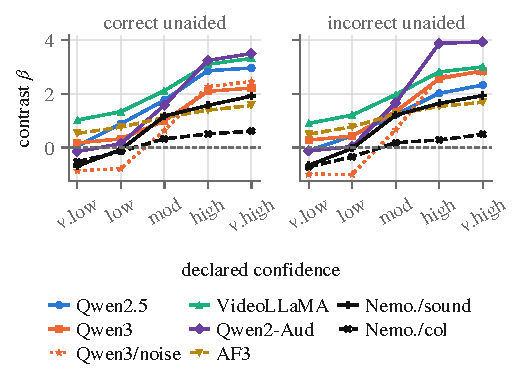
\includegraphics[width=\linewidth]{figures/fig1.pdf}
\caption{Claim-aligned $\beta$ (log-odds) versus declared confidence on unaided-correct items (left) and their
unaided-incorrect complements (right), using the first answer order. Left $n=308$--382; right $n=18$--92
(Qwen2.5/Qwen3 sound: 19/18). AF3 (dashed) is order-sensitive.}
\label{fig:decomp}
\end{figure}

$\beta$ rises monotonically with declared confidence in every one of the $\BetaPrimN$ ladder cells and in Audio Flamingo~3, reaching $+\BetaTopMin$ to $+\BetaTopMax$ at the top rung. At very low declared confidence, the claim-aligned contrast is negative in the Nemotron, Qwen2-Audio, and Qwen3/noise cells. The response is also damped: on the numeric scale, where the value is explicit, $\beta$ is close to linear in $\mathrm{logit}(c)$ ($R^2\ge\RsqMin$) with slope $\SlopeMin$--$\SlopeMax$, where a calibrated independent sensor taken at face value would give one.

We next test a restricted common-shift account. Because conditioning on unaided-correct items makes the baseline margin positive, output shrinkage can mimic the observed signs. Under the restricted null, a confidence-dependent term shared by the true- and false-claim branches cancels in $\beta$, predicting no complement swing. The swing persists under the prespecified first order (Fig.~\ref{fig:decomp}, right) and, in the two cells rerun in the swapped order (Qwen2-Audio, Nemotron/sound), there too: the complement's top-minus-bottom swing is $\EThreeSwingQTwoA$ and $\EThreeSwingNemo$ log-odds, both intervals above zero and the latter larger than in the first order. Rescaling common to both branches is not excluded by this test; the Priority control shows that a generic graded-value effect is insufficient.

The symmetric contrast $\alpha$ does not survive the complement analysis: it reverses sign in six of seven ladder cells and is therefore reported descriptively.

\begin{table}[tb]
\caption{Override rate (macro-POR, \%) under high vs.\ low declared confidence, order-averaged. $|C|$ counts items answered correctly unaided, per order; spread is the across-order range at high/at low. $p$ is the exact McNemar of the worse order, raw; Holm over the $K{=}\PorK$ prespecified per-order comparisons rejects $\PorRejN$.}
\label{tab:conf}
\centering\small
\setlength{\tabcolsep}{1.9pt}
\begin{tabular}{llrrrrl}
\toprule
model & cell & $|C|$ & high & low & spread & $p$ \\
\midrule
\TabPOR
\midrule
\multicolumn{7}{l}{fails admission in one order --- sensitivity only}\\
\TabPORsens
\bottomrule
\end{tabular}\\[2pt]
{\small $N{=}400$/order; $A_0{=}|C|/400$. $^{c}$ceiling $>0.95$ ($\text{-}1$/$\text{-}2$: first/swapped order). Cells without POR headroom are not rows.}
\end{table}

\subsection{Ablations}
\label{sec:robust}

Withholding the clip raises the contrast in $\MaskRiseN$ of $\MaskTotN$ masked cells, and outside the gate $\beta$ runs $\FloorMin$--$\FloorMax$, above the admitted maximum at high ($\EligMax$) in $\FloorAboveN$ of $\FloorN$ floor cells, indicating larger contrasts in several screened cells with weak unaided performance. The POR contrasts in Table~\ref{tab:conf} persist under a reworded question on the two Qwen sound cells ($\ParaMin$--$\ParaMax$\,pp).

\begin{table}[tb]
\caption{The $\LedgerTotN$ headline cells and the Audio Flamingo~3 sensitivity row. $A_0$ is unaided accuracy (\%), order-averaged; $\beta_{\mathrm{C}}$/$\beta_{\mathrm{P}}$ are the high-minus-low swings of $\beta$ under Confidence and Priority (log-odds), $\Delta$ their order-averaged paired difference with a source-clustered $95\%$ interval (393--399 videos, $2000$ replicates; within-order per-item s.d.\ $\DeltaSdWMin$--$\DeltaSdWMax$). $^{c}$: an order exceeds $0.95$. $^{s}$: sensitivity. g4: strongest graded-noise level.}
\label{tab:ledger}
\centering\small
\setlength{\tabcolsep}{2.5pt}
\begin{tabular}{@{}llrrrl@{}}
\toprule
model & attribute & $A_0$ & $\beta_{\mathrm{C}}$ & $\beta_{\mathrm{P}}$ & $\Delta$ [$95\%$ CI] \\
\midrule
\HeadRows
\bottomrule
\end{tabular}
\end{table}

The sound-event analysis includes $\LedgerSoundN$ cells (Table~\ref{tab:ledger}); the additional four colour and two noise cells show that the field-name contrast is not confined to sound-event questions. Inverting the options preserves the effect direction but not its magnitude --- Qwen3/noise's largest gap moves $\OrdGapO\to\OrdGapS$ --- so all both-order numbers are order-averaged. VideoLLaMA2.1's unaided sound accuracy falls to chance ($\VLSwapAcc$) under the swap, so those cells fail the gate there and are not reported.

\section{Cascade Evaluation}
\label{sec:policy}

\subsection{Detector and Forwarding Setup}

\begin{table*}[t]
\caption{A real cascade, order-averaged. CLAP~\cite{clap2023} tags each clip and its decision becomes the claim. $\pi^{\star}$ is the in-block break-even. Brackets are source-clustered $95\%$ intervals; the in-block ones (not shown) also exclude zero. $^{s}$: sensitivity.}
\label{tab:cascade}
\centering\small
\setlength{\tabcolsep}{2.1pt}
\begin{tabular}{lr rl rrr r}
\toprule
 & & \multicolumn{3}{c}{forward claim ($\Delta$ omit, pp)}
& \multicolumn{2}{c}{field ($\Delta$ block, pp)} & \\
\cmidrule(lr){3-5}\cmidrule(lr){6-7}
model & omit (\%) & \multicolumn{2}{c}{bare} & in block & verbal & numeric & $\pi^{\star}$ \\
\midrule
\TabCascade
\bottomrule
\end{tabular}
\end{table*}

CLAP (clap-htsat-unfused) scores each clip against the query class verbatim, unlike fixed-vocabulary taggers~\cite{gong2021ast}. Its threshold and band precisions are cross-fitted over a five-fold split of the source videos, and everything below is pooled over the five held-out folds, reaching $\DetAcc\%$ (per-fold s.d.\ $\DetFoldSD$).

CLAP’s raw similarity is neither calibrated nor thresholded at 0.5, so $\max(s,1-s)$ is not a confidence estimate for the emitted decision. We therefore fit $p=P(y=1\mid s)$ by isotonic regression and set \(q=p\) or \(1-p\) according to the emitted decision. For each held-out source-video fold, the isotonic map, decision threshold, and band boundaries are estimated from the remaining folds. The bands (training-fold quintiles of $q$) rise out-of-fold ($\BandMin$--$\BandMax\%$). All $\CasNumCells$ cascade cells are sound events.

For a fixed serialization, let $G_{\mathrm{true}}$ and $G_{\mathrm{false}}$ denote accuracy changes relative to
omission under true and false claims; mixing at claim correctness $\pi$ gives $\pi^{\star}=-G_{\text{false}}/
(G_{\text{true}}-G_{\text{false}})$. A true claim already costs $\CasTrueCostMin$--$\CasTrueCostMax$ points in
$\CasNoBreakEven$ of $\CasNumCells$ cells, so those claim-only policies have no feasible break-even. All cascade
cells are predicted to lose, and the $\CasPrimN$ order-robust rows do by $\CasLossMinP$--$\CasLossMaxP$ points
(Table~\ref{tab:cascade}). Because claim errors depend on item difficulty, $\pi^{\star}$ is approximate; recommendations use the measured outcomes.

Bare forwarding costs $\KillMin$--$\KillMax$ points in every order-robust cell. The loss replicates at a second CLAP checkpoint ($\KillMinB$--$\KillMaxB$ points) and in all $\FamCells$ cells tested with Qwen2-Audio as detector
($\FamMin$--$\FamMax$ points); all prespecified bare-cascade tests remain significant after Holm correction. Post hoc, false absences account for $\DirFNShareMin$--$\DirFNShareMax\%$ of the false-claim loss.

\begin{figure}[h]
\centering
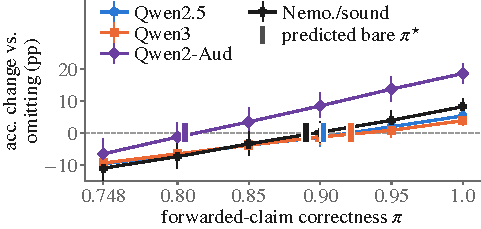
\includegraphics[width=\columnwidth]{figures/fig2_sweep_v2.pdf}
\caption{Error-repair sweep. Bare-forwarding accuracy change relative to omission versus target forwarded-claim correctness $\pi$; the leftmost point is the observed CLAP operating point. Error bars are source-clustered $95\%$ intervals, and ticks mark the predicted bare-sentence break-even $\pi^{\star}$ (Table~\ref{tab:cascade}: in-block $\pi^{\star}$).}
\label{fig:sweep}
\end{figure}

\subsection{Break-Even and Serialization}
One seeded subset of the detector's errors is corrected per fold, with the real run and the wholly true claim as endpoints. This keeps the clip, question, and reader fixed while changing only which detector errors are converted into true claims. Accuracy crosses zero $\CrossGapMinPP$--$\CrossGapMaxPP$\,pp above the predicted bare $\pi^{\star}$, with intervals covering zero in all $\GapZeroN$ cells; two further seeds place $\SeedAgreeCells$ of $\SeedTotCells$ crossings in the same grid interval (Fig.~\ref{fig:sweep}). The separated crossings show that break-even is reader-specific rather than a property of detector correctness alone. At the observed CLAP point all four curves lie below zero; Qwen2-Audio, the weakest unaided reader among the order-robust cells, has the lowest predicted threshold.

A stronger cross-fitted probe reverses Qwen2-Audio ($\StrongQTwoA$ [$\StrongQTwoALo$, $\StrongQTwoAHi$] points),
while its accuracy remains below the two Qwen-Omni break-even thresholds. Near Nemotron's estimated threshold, the interval includes zero and does not confirm the prespecified positive sign. All estimates lie within $\ProbeSweepMax$\,pp of the sweep prediction. Qwen2-Audio's cascade then approximately matches the probe's own accuracy, showing that the gain is over the reader rather than the detector.

\looseness=-1
The Source/Claim block attenuates the claim response: across the $\PackPrimBelowN$ order-robust cascade cells, the
true--false gap falls to $\PackPrimMin$--$\PackPrimMax\%$ of the bare span (median $\PackPrimMed\%$), with both directions shrinking. Across the $\PackColCells$ colour cells, the gap falls to $\PackColMin$--$\PackColMax\%$ of the bare span (median $\PackColMed\%$). Audio Flamingo~3 illustrates that attenuation is not itself an accuracy gain: its gap shrinks, yet block accuracy worsens by $\AFBlockGap$ points and it fails the order gate. The recommendation is therefore limited to order-robust readers.

The attenuation is not a free gain: under true claims, the no-field block costs $\FrameMin$--$\FrameMax$ points, while adding Confidence recovers $\FieldMin$--$\FieldMax$ points, with intervals above zero in $\FieldPosN$ cells. On the first-order ladder, numeric confidence reduces the verbal very-low-to-high swing to $\CompressPrimMin$--$\CompressPrimMax\%$. In the cascade, band-precision numbers improve on verbal confidence by $\CasNumGainMin$--$\CasNumGainMax$ points in every tested cell. Against the no-field block, numeric confidence improves $\NumOverBlockN$ of $\NumBlockCells$ cells, ties one, and worsens $\NumUnderBlockN$.

A disclaimer helps in only $\EFourWarnPosN$ of $\EFourCells$ cells, and all still trail omission. The block
matches or improves bare forwarding in all $\EFourCells$ cells; an oracle confidence gate, with its threshold selected on the test set, gains at most $\SelGainMax$ points (descriptive). Because its threshold is test-selected, this is an optimistic upper bound on confidence-only routing.

\looseness=-1
The confidence-field effect is smaller than claim insertion but exceeds the Priority control in every headline cell. On accuracy, exploratory intervals exclude zero in $\ConfAccSigN$ of $\ConfAccCells$ cascade cells; in
\FieldOverClaimCell{}, the field effect even exceeds the in-block claim.

\section{Limitations}
\label{sec:limits}

\looseness=-1
All six readers are open and ${\le}30$B; five use Qwen-family text backbones, Nemotron differs in its listed components, and all cells come from one corpus. The order-robust admitted cells have higher unaided accuracy than CLAP, while the only separately reported below-CLAP cell fails the order gate; costs are therefore measured mainly in a strong-reader/weak-detector regime. The stronger probe reverses one reader's outcome, so the policy is detector--reader specific. In an audit of $\AuditN$ clip--query pairs with judgments recorded independently, $\AuditAgree\%$ of definite judgments agree with the query labels; removing disagreements and unsure cases leaves a $\CleanMin$--$\CleanMax$-point bare loss.

\section{Conclusion}
\looseness=-1
At the original CLAP operating point, omission outperformed all unconditional text-forwarding policies in the four order-robust cells; a stronger probe reversed this result for one reader, consistent with the estimated break-even. Among order-robust readers, the Source/Claim block matched or improved bare forwarding. Numeric confidence was less harmful than verbal confidence, though not consistently better than omitting the field. Forwarding should therefore be calibrated for each detector--reader--serialization tuple.

\clearpage

\section{Compliance with Ethical Standards}
This study uses publicly available datasets and pretrained models and involves no newly recruited human or animal participants.

\section{Acknowledgements}
This work was supported by the Institute of Information \& Communications Technology Planning \& Evaluation (IITP) grant funded by the Korea government (MSIT) (No.~RS-2024-00438027, Development of an intelligent security and risk response system based on multi-modal data integration analysis), and by the IITP under the Artificial Intelligence Innovation Human Resources Development grant (IITP-RS-2026-25547954) funded by the Korea government (MSIT). The authors declare no relevant conflicts of interest.

\bibliographystyle{IEEEbib}
\bibliography{refs}
\end{document}
